\documentclass[spanish]{article}
\usepackage[T1]{fontenc}
\usepackage[utf8]{luainputenc}
\usepackage{amsmath}
\usepackage{amssymb}
\usepackage{graphicx}

% packages
\usepackage{xspace}
\usepackage{ifthen}
\usepackage{amsbsy}
\usepackage{amssymb}
\usepackage{balance}
\usepackage{booktabs}
\usepackage{graphicx}
\usepackage{multirow}
\usepackage{needspace}
\usepackage{microtype}
\usepackage{bold-extra}
\usepackage{subfigure}
\usepackage{wrapfig}
\usepackage{enumerate}

% references
\usepackage[colorlinks]{hyperref}
\usepackage[all]{hypcap}
\setcounter{tocdepth}{2}
\hypersetup{
        colorlinks=true,
        urlcolor=black,
        linkcolor=black,
        citecolor=black,
        plainpages=false,
        bookmarksopen=true,
        pdfauthor={Alvaro Jose Peralta Ocampo},
        pdftitle={Titulo}}


\makeatletter
%%%%%%%%%%%%%%%%%%%%%%%%%%%%%% User specified LaTeX commands.
\usepackage{babel}




\usepackage{babel}
\addto\shorthandsspanish{\spanishdeactivate{~<>}}



\makeatother

\usepackage{babel}
\addto\shorthandsspanish{\spanishdeactivate{~<>}}





% proof-reading
\usepackage{xcolor}
\usepackage[normalem]{ulem}
\newcommand{\ra}{$\rightarrow$}
\newcommand{\ugh}[1]{\textcolor{red}{\uwave{#1}}} % please rephrase
\newcommand{\ins}[1]{\textcolor{blue}{\uline{#1}}} % please insert
\newcommand{\del}[1]{\textcolor{red}{\sout{#1}}} % please delete
\newcommand{\chg}[2]{\textcolor{red}{\sout{#1}}{\ra}\textcolor{blue}{\uline{#2}}} % please change
\newcommand{\chk}[1]{\textcolor{green}{#1}} % changed, please check

% comments \nb{label}{color}{text}
\newboolean{showcomments}
\setboolean{showcomments}{true}
\ifthenelse{\boolean{showcomments}}
        {\newcommand{\nb}[3]{
                {\colorbox{#2}{\bfseries\sffamily\scriptsize\textcolor{white}{#1}}}
                {\textcolor{#2}{\sf\small$\blacktriangleright$\textit{#3}$\blacktriangleleft$}}}
         \newcommand{\version}{\emph{\scriptsize$-$Id$-$}}}
        {\newcommand{\nb}[2]{}
         \newcommand{\version}{}}
\newcommand{\rev}[2]{\nb{Reviewer #1}{red}{#2}}
\newcommand{\ab}[1]{\nb{Alexandre}{blue}{#1}}
\newcommand{\ai}[1]{\nb{Alejandro}{orange}{#1}}
\newcommand{\on}[1]{\nb{Oscar}{olive}{#1}}



\begin{document}



\title{Propuesta de tesis Magíster TI \ab{Give a better title. Cual es el titulo de tu trabajo?} }


\author{Universidad de chile, DCC}


\author{Alvaro Jose Peralta Ocampo}


\date{Mayo 2014}

\maketitle

\section{Introducción}

En el contexto empresarial la constante que más resalta es la variabilidad
de los procesos de negocio que es ocasionada por la dinámica de crecimiento
constante y mejora continua a la que las organizaciones están sometidas
en un ambiente de alta competitividad. Realidades del negocio como
fusiones corporativas, cadenas de valor distribuidas, nuevas tecnologías,
nuevas formas de negocio, clientes formados tecnológicamente. Ha ocasionado
requerimientos muy exigentes al área de TI que día a día se ve afrontada
a brindar soluciones innovadoras, en menor tiempo con menor costo
de inversión \cite{libroInteroperabilidadDCC2009}.

Este hecho fundamental ha generado toda una industria que durante
el principio de este siglo ha florecido por presentar una solución
profesional dentro de esta dinámica heterogénea de operaciones altamente
interconectadas, de requerimientos cambiantes con una alta necesidad
de reutilización de factores críticos de éxito.

Esta solución propuesta por la industria es conocida actualmente como
``Arquitecturas Orientadas a Servicio”, solución que viene siendo
la principal respuesta para lograr coordinar la dinámica en la interacción
de los diferentes actores que son involucrados en la cadena de valor
de las organizaciones. Su principal objetivo es la reutilización de
``servicios” que ya funcionan en la organización disminuyendo así
la complejidad en la integración de procesos.

Esta coordinación es desarrollada básicamente por dos conceptos elaborados
en el contexto SOA denominados orquestación y coreografía que cumplen
un papel análogo a su definición natural permitiendo que los actores
logren completar cierta sinergia gracias a la elaboración de flujos
de trabajo desarrollado por el esfuerzo conjunto entre el área de
TI y de negocio que en adelante llamaremos procesos de negocio web.

Estos procesos de negocio no son muy diferentes de los denominados
workflows o flujos de trabajo, representan más bien una evolución
tecnología. Mientras que los workflows invocan tareas, los procesos
web invocan servicios web \cite{Cardoso2008}.

Al parecer la facilidad con que estos procesos de negocio son desarrollados
y mantenidos gracias al uso de lenguajes estandarizados por la W3C
como por ejemplo: (WS-BPEL 2005). Que es implementado en soluciones
SOA lo que ha generado un gran adelanto tecnológico en la relación
Negocio-TI.

Sin embargo la realidad de ``adaptación al cambio constante” no ha
cambiado en su esencia misma, ocasionando que cada vez más los procesos
de negocio sigan evolucionando y ampliando su complejidad tanto en
requerimientos funcionales como no funcionales, por lo que aun teniendo
una arquitectura tan robusta como lo es la propuesta en el contexto
SOA los atributos de calidad del software que aún se aplican en lenguajes
como BPEL siguen siendo una preocupación tanto para el área de TI
como para el negocio en sí mismo.

Este propuesta de tesis relata en su punto numero 2 porque el desarrollo
de procesos de negocio es complejo y lleno de preocupaciones asociadas
a la complejidad y calidad en la construcción de dichos procesos,
definiendo así un conjunto de problemas que son los que mas sobresalen
durante un ciclo de vida normal de construcción.

Una ves argumentado y listado el grupo de problemas se describe de
manera muy resumida en el punto numero 3 las distintas disciplinas
de ingeniería y gestión que son necesarias para abordar el desafió
de construir una herramienta para la valoración de procesos de negocio
en el lenguaje ( BPEL ) finalizando así con el punto 4 y 5 con una
declaración formal de lo que se pretende entregar al finalizar el
proyecto de tesis junto con un breve resumen de las macro actividades
que se han estado realizando a la fecha de entrega de esta propuesta. 


\section{Problema a resolver / Oportunidad de Mejora}

\emph{Contexto:} Análisis de procesos de negocio orientados a la web
en situaciones de alta complejidad con requerimientos funcionales
cambiantes en un entorno de arquitecturas orientadas a servicio.

\ab{Larga farsa. hay que usar puntos} La oportunidad de mejora se centra en lo que hemos llamado ``complejidad
de procesos de negocio web” debido a que esta se produce en el proceso
de desarrollo no está exenta de los mismos problemas al construir
un software tradicional, por ejemplo: inyección de defectos, excepciones
inesperadas, poca comprensión del proceso. Lo que a este nivel de
abstracción puede ser un costo tremendo tanto el proceso de desarrollo
como en el impacto en el negocio.

Tomemos como ejemplo el caso de estudio que propone la suite de Oracle
SOA Suite, de nombre Fusion Order Demo {[}2{]} que simula el comportamiento
de una empresa internacional de retail como Fallabela o París conocidas
en el contexto chileno.

El servicio que nos interesa observar del ejemplo puntualmente es
la ejecución del proceso de orden de compra, siendo este el flujo
de proceso que se necesita para llevar a cabo una compra de un grupo
de ítems previamente seleccionados de un carrito de compras hasta
su envió y notificación al cliente de que su orden le ha sido enviada
por un proveedor de transporte físico.

Para lograr este objetivo el proceso de negocio tiene que interactuar
con múltiples actores dentro de la cadena de valor además de ejecutar
ciertas instrucciones de negocio para determinar para producir el
flujo esperado.

Suponiendo que esta introducción sea una reunión inicial que el área
de TI tenga con el área de negocio para su nuevo proyecto SOA. Nuestro
equipo se ve obligado a definir una propuesta de alcance, partiendo
de su experiencia y de métricas de procesos similares, pero:

\vspace{0.5cm}
\textbf{\emph{Problema 1 - Ausencia de métricas como complejidad,
calidad, portabilidad entre otras}}

Al no tener métricas recolectadas de procesos anteriores o en su defecto
no poder dimensionar métricas de procesos ejemplo, No se puede estar
seguro del tamaño y/o complejidad de lo que se nos está pidiendo,
este ha sido un problema recurrente y estudiado en varias publicaciones
como \cite{Cardoso2008,Cardoso2006,Budnik2011}, los cuales proponen
distintas formas de medir procesos BPEL.

Debido al primer problema encontrado, la propuesta de alcance se construye
desde la labor heurística del arquitecto líder, que puede prometer
cualidades del software que no lo comprometan. Por ejemplo: Un grado
de mantenibilidad del 80\% y una complejidad MEDIA de la lógica del
proceso. Medidas que para la promesa de la arquitectura SOA son totalmente
inadecuadas.

El caso inicial de la primera iteración nos llevara a construir un
proceso de negocio que en términos de \emph{calidad} dependerá de
cuan avanzados estemos como organización en los \emph{niveles de madures
SOA\cite{IBMSOAG2006}} , por lo que en niveles bajos: \ab{Porque ``:''? La frasa no parece ser terminada}

\vspace{0.5cm}
\textbf{\emph{Problema 2 - Dificultad en la estimación de esfuerzo}}

Al no tener definido un marco de trabajo con el que podamos valorar
características inherentes al software BPEL (Proceso de negocio),
tendremos poca visualización en varias perspectivas de la calidad
de nuestro desarrollo, por ejemplo Budnik \cite{Budnik2011} menciona
preocupaciones como productividad , reducción de costos y riesgos
entre otras.

Llegados a este punto la confianza del área de negocio en el éxito
del proyecto radica en la habilidades humanas que entregan los consultores
SOA al equipo de desarrollo, que para este caso contextual finalizan
el proceso, entregando un proceso probado finalizando así su compromiso
con el proyecto.

\vspace{0.5cm}
\textbf{\emph{Problema 3 - Actividades de validación de pruebas insuficientes}}

Para el arquitecto de TI junto con el área de QA los cuales, tiene
la responsabilidad de recibir dichas pruebas. Deben valerse de herramientas
como inspecciones de código para poder decidir si hay completitud
y suficiente esfuerzo de pruebas que validen la de los consultores
y/o implementa dores de procesos. Lo que se convierte en una actividad
que agrega esfuerzo adicional al proyecto, Lubke and Singer \cite{DanielLubke2009}
comparten el problema al proponer un mecanismo para verificar cobertura
de pruebas realizadas a los procesos BPEL, propuesta que es un problema
complementario dentro de esta gran preocupación que es la calidad.

Continuando con la característica mencionada en la introducción de
esta propuesta de tesis que hace referencia a la constante ``cambio”
en el negocio, los estudios indican que el 38\% de las soluciones
con procesos de negocio se les aplicara un proceso de rediseño en
toda la organización (Delphi Group, 2002)\ab{Hay que usar solamente uno estillo de referencia} \cite{Cardoso2008}, por
lo que una perspectiva cíclica de constantes proyectos de desarrollo
es aplicable constantemente en este ambiente de servicios y procesos.
Esto sumado a la complejidad en la gestión de requisitos, principalmente
debido a que la infraestructura en la que se implementan los procesos
BPEL, esta dotada de \emph{indicadores de proceso} que permiten ajustar
los procesos con base en su historial de desempeño, echo que motiva
a los ingenieros de proceso a generar nuevas actividades tanto en
la revisión del proceso en producción como en la etapa de creación
del proceso. lo cual agrega un nuevo problema dentro de los actuales
análisis de procesos con los que cuentan las herramientas y es que:

\vspace{0.5cm}
\textbf{\emph{Problema 4 - Indicadores estáticos y dinámicos insuficientes
para detectar anormalidades}}

Muchos de los indicadores son de análisis dinámico (es decir métricas
que se toman mientras el proceso es ejecutado), solo se alcanzan a
medir en escenarios de alto nivel, entregando indicadores de caja
negra. Por lo que estos indicadores No alcanzan a revelar causas dentro
del contenido de los procesos. Siendo este problema parte de las actividades
de análisis dinámico de procesos, tal como lo menciona Budnik \cite{Budnik2011}
y también Chang and Lee \cite{Chang2009}. Donde menciona criterios
de calidad de servicios que son aplicables para el desempeño en procesos
BPEL.

Hasta este punto hemos visto que nuestras preocupaciones se centran
en medir, evaluar y validar la correcta producción de procesos de
negocio dentro de un ambiente controlado y orquestado por una área
de procesos la cual debe preocuparse por gobernar una arquitectura
muy compleja organizacionalmente, la figura.\ref{fig:Preocupaciones-del-Govierno}
muestra el contexto básico por lo que debe preocuparse un gobierno
de servicios: Quien toma las decisiones y ejecuta los procesos, que
políticas se deben aplicar en los procesos, ejemplo: timeout y de
no repudiación y por ultimo como todo este ambiente es orquestado
y controlado por los procesos.

\begin{figure}
\centering{}\caption{ \label{fig:Preocupaciones-del-Govierno}Preocupaciones del Gobierno
SOA\cite{Weir2013}}


\raggedright{}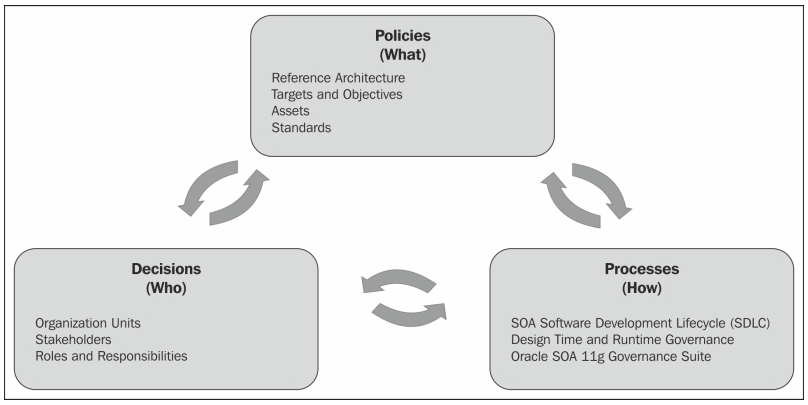
\includegraphics[scale=0.6]{img/SOAGovernanceConcerns} 
\end{figure}


El gobierno de procesos es importante en este punto para destacar
que si bien todos los problemas anteriormente mencionados están siendo
trabajados en distintos centros de investigación los cuales están
produciendo herramientas metodológicas para mejorar cada problema
lo cual es una gran avance. Sin embargo la inversión que es necesaria
para que estas preocupaciones sean mitigadas es muy alta, similar
a la inversión que se necesita en un desarrollo de software tradicional
para realizar análisis,

\vspace{0.5cm}
\textbf{Problema 5 - Realizar valoración de procesos BPEL requiere
un enorme esfuerzo}
\ab{Este titulo no tiene el mismo formato que los otros t�tulos de problemas}

por tanto una valoración de software ( procesos BPEL incluidos) es
costosa y necesita de re-ingeniería \cite{Girb2011}, Además requiere
de múltiples herramientas que solucionan cada preocupación por separado
, por lo que se requiere de varios profesionales especializados por
cada disciplina a mitigar.

Podemos entender en este punto que las iniciativas de mejora en el
área de los lenguajes para definir procesos de negocio son un tema
que continua desarrollándose, que necesita de herramientas, métricas
y metodologías que aporten el desarrollo de mejores procesos, dentro
de las cualidades de software requeridas por el negocio.

\vspace{0.5cm}
\textbf{Problema 6 - Disciplina de valoración no es comunmente adoptada
en el proceso de desarrollo de procesos BPEL}

En ambientes empresariales estos esfuerzos independientes aun no han
sido integrados a la metodología de trabajo en desarrollo de procesos,
por lo que el esfuerzo en tiempo, costo y capital humano es muy significativo.

Se ha demostrado en otros contextos del desarrollo de software que
contar con herramientas que permitan visualizar diferentes perspectivas
de arquitectura son una excelente manera de integrar la valoración
del producto al ciclo de vida del desarrollo, caso de ejemplo es \url{www.moosetechnology.com}.
Herramienta que tiene como propósito incrementar las opciones y la
productividad de las valoraciones de software utilizando múltiples
herramientas que permiten analizar las diferentes perspectivas de
un software siendo el aspecto mas importante la capacidad de co-crear
nuevas formas de análisis adaptadas a contextos específicos.

De esta forma si aplicamos el mismo concepto a desarrollo de procesos
de negocio en particular a procesos BPEL tendremos la oportunidad
de tener una plataforma en la que podamos integrar las distintas preocupaciones
que nos habiliten mejores análisis dentro de procesos de desarrollo
de software orientados a procesos de negocio en la WEB.


\section{Justificación de la propuesta}

El propósito de esta tesis se centra en la mejora de la calidad del
software orientada a procesos desarrollados en BPEL bajo el contexto
SOA, pero dado el nivel estratégico que tiene dicha arquitectura y
su alto impacto que tiene esta en la relación del negocio con el área
de TI las actividades y herramientas que sean propuesta en este trabajo
de tesis involucran también propuestas en el proceso de desarrollo
como parte integral de producir una herramienta de valoración de código
BPEL.

El constante crecimiento de esta tecnología, principalmente ahora
en donde la dinámica de la industria ha permitido que la arquitectura
SOA pueda ser implementada con menos costos operativos, ha generado
una gran demanda por mejores estrategias para una correcta gestión
del proceso como del desarrollo tanto en la gran industria como en
la mediana industria.

Ahora es normal ver como empresas pueden usar infraestructuras en
la nube para usar esta tecnología con costos muy competitivos y de
fácil acceso, lo cual ha generado una gran expectativa en términos
de integración con otros negocios y nuevas formas de hacer servicios.

En la medida que se agregue complejidad a estos procesos, las actividades
de evaluación y mejora de la calidad se hacen mas evidente, por lo
que aportar con una herramienta que ayude a los ingenieros a desarrollar
mejores procesos de negocio generar un enorme valor agregado, principalmente
porque busca definir una infraestructura con en la que se puede seguir
avanzando en la investigación y en el desarrollo de nuevas formas
de valoración de procesos negocio en la web.

Para poder cumplir con el objetivo principal es necesario utilizar
todas las disciplinas asociadas a la ingeniería del software, adicionando
un especial esfuerzo a la disciplina de análisis y diseño en términos
de arquitectura dado que el principal objetivo es permitir a los ingenieros
validar si sus diseños cumplen con las expectativas de los requisito
del negocio.

El principal desafió de este proyecto se centra en construir herramientas
que \emph{visualmente permitan a el equipo de desarrollo tomar mejores
decisiones con respecto al diseño de sus procesos de negocio}, lo
cual conlleva realizar un arduo trabajo de investigación en el estado
del arte en indicadores, complejidad del proceso,evaluación,ciclos
de vida y de maduración en procesos BPEL como en implantación del
paradigma SOA.


\section{Objetivo General}

Diseñar e implementar de una herramienta que permita la valoración
y el análisis del diseño de procesos de negocio construidos en BPEL
de forma estática.


\subsection{Objetivos Específicos}
\begin{itemize}
\item Diseñar e implementar un mecanismo de navegación y valoración de los
diferentes componentes de procesos de negocio BPEL dentro de un contexto
SOA. 
\item Diseñar e implementar una herramienta que permita de manera flexible
generar nuevas visualizaciones de complejidad en proceso de negocio
y sus indicadores dentro de la suite de trabajo moosetechnology. 
\item Investigar y/o elaborar al menos 2 indicadores por cualidad de software
relevante en la elaboración de procesos de negocio web. 
\item Definir un proceso metodológico básico que permita realizar valoración
de procesos de negocio construidos en BPEL usando la herramienta como
eje fundamental de trabajo. 
\item Aplicar el proceso metodológico propuesto de valoración de procesos
web dentro de un contexto organizacional que de como resultado documento
de mejora a procesos BPEL. 
\end{itemize}



\section{Metodología / Plan de trabajo}

Ha la fecha de entrega de este documento ya se ha iniciado con una
fase de concepción en donde se ha realizado una evaluación de la suite
de trabajo moosetechnology como herramienta principal de co-creación
de la herramienta. Observando que existen numerosas ventajas, para
el análisis y principalmente para la producción de herramientas de
vizualización y navegabilidad de artefactos.

Con base en el éxito de esta primera fase en la que principalmente
se realizaron tareas utilizando una estrategia de metodología ágil
guiada por paquetes de trabajo cortos y validación, con la que efectivamente
se verifico la viabilidad de la propuesta de tesis, ademas de que
siendo este proyecto es una propuesta netamente de innovación. Se
concluye que optar por una estrategía iterativa e incremental guiada
por una herramienta de gestión tipo scrum es la que mas se ajusta
a este modelo.

\textbf{Plan de trabajo General - Macroactividades}
\ab{Quizas agregar una carta gantt para ver los progresos y tiempo de cada cosa?}
\textbf{Seminario de tesis 1} 
\begin{itemize}
\item Estudiar y dominar las bases del desarrollo bajo la plataforma moosetechnology. 
\item Estudiar y definir los diferentes indicadores y métricas que existen
hasta la fecha para la complejidad de procesos BPEL 
\item Elaborar requisitos de usuario con base en la investigación y necesidades
recolectadas. 
\item Producir el documento de avance de tesis. 
\item Realizar charla de avance tesis I 
\item Desarrollar y probar la versión preliminar de la herramienta. 
\end{itemize}
\textbf{Seminario de tesis 2} 
\begin{itemize}
\item Realizar pruebas asociadas a varios escenarios de negocio donde se
usan procesos BPEL. 
\item Definir el conjunto de actividades en donde la herramienta es de alta
utilidad. 
\item Diseñar el flujo de actividades en donde la metodología puede ser
implementada bajo el modelo de Madurez SOA. 
\item Elaborar propuestas alternativas de análisis con base en nuevas herramientas
de desarrollo por ejemplo lenguaje de aspectos en BPEL. 
\item Realizar una valoración profesional en un contexto SOA donde se implementen
procesos BPEL. 
\item Producir el documento final de tesis. 
\item Realizar defensa de tesis ( Charla de tesis II ) 
\end{itemize}
 \bibliographystyle{plain}
\bibliography{MGTI}
 
\end{document}
